% -*- mode: latex-mode; TeX-engine: xetex; LaTeX-command-style: (("" "SOURCE_DATE_EPOCH=0 %(PDF)%(latex) --shell-escape %S%(PDFout)")); TeX-master: "../dissertation.tex"; -*-

\chapter{Coherent Optical Creation of NaCs Molecule}
\label{ch:raman-transfer}

\section{Introduction}
\label{ch:raman-transfer:introduction}

The coherent production of weakly bound ground state NaCs molecule is an important milestone
in our two-step approach of creating rovibronic ground state molecules with full control.
Achieving this goal using only optical transition without a narrow excited state linewidth
can allow more laser-coolable atoms to be associated to molecules coherently.
With the characterization of both the excited and ground molecular potential,
we have calibrated all the parameters needed to drive such a transition.
Nevertheless, the wavefunction size mismatch between the atomic and molecular states
remains a challenge that requires careful selection of the transition pathway.

In this chapter, we will discuss the considerations behind our choice of parameters
and show the result of the coherent molecule creation.
We begin with section~\ref{ch:raman-transfer:raman} to setup a model
for a realistic Raman transition beyond the ideal three-level system.
Section~\ref{ch:raman-transfer:stirap} follows a similar track and constructs a model
for stimulated Raman adiabatic passage~(STIRAP),
which is another common way to drive such a two-photon transition
and comparing it to the Raman transition.
Section~\ref{ch:raman-transfer:state-selction} uses the result from the previous sections
to finalize our molecule creation pathway.
The result of the molecule creation is given in section~\ref{ch:raman-transfer:results},
which also includes discussion on the transfer efficiency.

\section{Raman Transition Beyond Three-Level Model}
\label{ch:raman-transfer:raman}

For a Raman transition with Raman Rabi frequency $\Omega_{\mathrm{R}}$ and total scattering rate
$\Gamma$, defined as the sum of the scattering rate for the initial and final states,
the probability of scattering during a $\pi$ pulse is,
\begin{align*}
  p_{\mathrm{s}}=&\frac{\Gamma t_{\pi}}{2}\\
  =&\frac{\pi\Gamma}{2\Omega_{\mathrm{R}}}
\end{align*}
which is proportional to the ratio $\Gamma/\Omega_{\mathrm{R}}$.
In an ideal three-level system, this is the only source of decoherence
which can be made arbitrarily small by using a large
single photon detuning~(section~\ref{ch:rsc:basic-theory:raman-scatter}).
However, in a real system, there are often other effects that increases the scattering
and may also put a lower limit on the scattering probability during the transfer.
Fig.~\ref{fig:raman-transfer:generic-raman-model} shows a generic model
for a real Raman transition demostrating some of these effects.
Additionally, other practical limitation in the system like stability of the laser power
and frequency also needs to be taken into account.

\begin{figure}
  \centering
  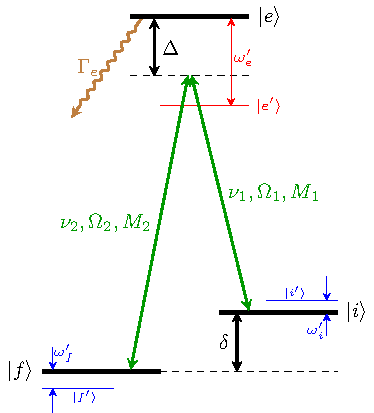
\includegraphics[width=0.6\textwidth]{figures/raman_transfer_generic_raman_model.pdf}
  \caption[Generic model for a real Raman transition]{
    Generic model for a real Raman transition.
    The initial state $|i\rangle$ and the final state $|f\rangle$
    has a energy difference $\delta$
    and are coupled by two Raman beams with frequencies and
    single photon Rabi frequencies of $\nu_1,\ \Omega_1$ and $\nu_2,\ \Omega_2$ respectively.
    The corresponding matrix elements (arbitrary unit) are $M_1$ and $M_2$.
    The Raman beams are detuned by $\Delta$ from the primary excited state $|e\rangle$,
    which has a decay rate of $\Gamma_e$.
    We also consider additional states near the initial~($|i'\rangle$),
    final~($|f'\rangle$) and intermediate excited $|e'\rangle$ states which are
    separated from the corresponding Raman transition states by $\omega'_i$,
    $\omega'_f$ and $\omega'_e$ respectively.
    Only one additional state of each kinds are included to simplify the discussion
    without loss of generality.
    \label{fig:raman-transfer:generic-raman-model}}
\end{figure}

In the experiment, we find the parameter range that gives the best transfer efficiency
using numerical simulation~(section~\ref{ch:raman-transfer:state-selction}).
Nevertheless, in order to develop a general approach that can be applied to other systems,
it is also important to understand the various physical mechanism that leads
to the optimal parameters.
Therefore, in this section, we will discuss some of the most important effects
on the transfer efficiency at qualitative and semiquantitative level.
Due to experimental constraint, we will assume that the single photon detuning is
much smaller than the frequency of each individual beams, i.e. $\Delta\ll\nu_1,\ \nu_2$.

\subsection{Additional Initial and Final States}
\label{ch:raman-transfer:raman:extra-init-final}

First, we will discuss the effect of $|i'\rangle$ and $|f'\rangle$ states
near the initial and final states.
These states can be coupled to the excited state $|e\rangle$ by the Raman beams,
which can in tern be coupled to the initial and final states
by an off-resonance Raman transition.
The leakage is suppressed by the detuning from the Raman resonance,
i.e. $\omega'_i$ and $\omega'_f$.
This puts a limit on the Raman Rabi frequency $\Omega_{\mathrm{R}}$ to be smaller
than the smallest energy gap, which in turns puts a limit on the minimum Raman transfer time.
In our experiment, the minimum energy gap comes from axial motional excitation of
the atomic initial states which is between $2\pi\times10 - 30~\mathrm{kHz}$
depending on the trap depth used.
The typical Raman $\pi$ time we can realize is $0.5 - 5~\mathrm{ms}$ so this effect
is not a major limiting factor for our transfer efficiency.

\subsection{Additional Excited States}
\label{ch:raman-transfer:raman:extra-ext}

\begin{figure}
  \centering
  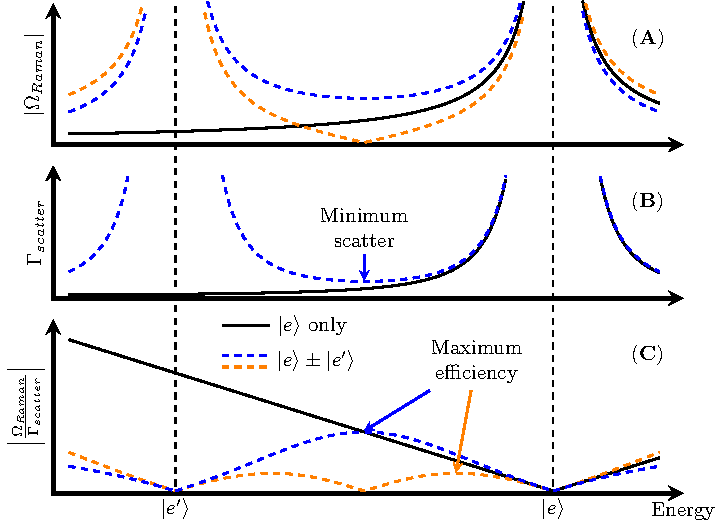
\includegraphics[width=\textwidth]{figures/raman_transfer_extra_ext_states.pdf}
  \caption[Raman transition with additional excited states]{
    Effect of additional excited states $|e'\rangle$ on the Raman transition efficiency.
    (A) Depending on the sign of the coupling, there could be constructive~(blue)
    or destructive~(orange) interference on the Raman Rabi frequency $\Omega_{\mathrm{R}}$.
    (B) Increased scattering rate $\Gamma_{\mathrm{s}}$ caused by $|e'\rangle$ with a minimal
    between the two states.
    (C) Optimal detunine exists between the two states with maximum transfer efficiency
    corresponds to a fraction of the state spacing.
    \label{fig:raman-transfer:raman:extra-ext-states}}
\end{figure}

Next, we will consider the effect of the $|e'\rangle$ state near the excited intermediate state.
These states can be coupled to the ground states, both $|i\rangle$ and $|f\rangle$,
by the Raman beams and can cause a change in both the Raman Rabi frequency
and the scattering rate.
There are two relevant limiting cases that needs to be discussed separately.

\subsubsection{Excited State Spacing Larger than Single-Photon Detuning}
\label{ch:raman-transfer:raman:extra-ext:large-spacing}
In this case, the single photon frequency falls in between the two excited states
$|e\rangle$ and $|e'\rangle$,
which happens when $|e'\rangle$ is a different vibrational or electronic state.
The total Raman Rabi frequency~(Fig.~\ref{fig:raman-transfer:raman:extra-ext-states}A) is,
\[
  \Omega_{\mathrm{R}}=\frac{\Omega_1\Omega_2}{2\Delta}+\frac{\Omega'_1\Omega'_2}{2(\Delta-\omega'_e)}
\]
where $\Omega'_1$ and $\Omega'_2$ are the single photon Rabi frequencies coupling $|e'\rangle$
to $|i\rangle$ and $|f\rangle$ respectively.
Depending on whether $\Omega'_1\Omega'_2$ has the same~(orange line)
or different~(blue line) sign as $\Omega_1\Omega_2$, the total Raman Rabi frequency
may be cancelled or enhanced between the two excited states.
On the other hand,
the total scattering rate~(Fig.~\ref{fig:raman-transfer:raman:extra-ext-states}B)
is almost always increased due to the additional state, creating a local minimum
between the excited states.
Combining the two effects, the ratio between the Raman Rabi frequency and
the scattering rate, which determines the transfer efficiency, always have local maximum
between the excited states~(Fig.~\ref{fig:raman-transfer:raman:extra-ext-states}C).

Despite the difference in the position and value of the maximum for different
$|e'\rangle$ parameters, we can summarize the effect on the transfer efficiency
as a limit on the maximum detuning $\Delta_{\max}$ to a fraction of the spacing
between the excited states~($\omega'_e$).
As an example, the blue and orange maxima in
Fig.~\ref{fig:raman-transfer:raman:extra-ext-states}C
corresponds to a limit on single photon detuning of $0.5\omega'_e$ and $0.15\omega'_e$.
As one would expected, a larger excited state spacing usually result in
a larger detuning limit and a better transfer efficiency.

Summarizing the effect of additional excited state as a single number $\Delta_{\max}$ allows
us to keep using the equation for Raman transition with minor corrections
and makes it easier to compare different state selection and transition schemes.
It is also worth noting that although only one additional excited state $|e'\rangle$
is considered here, this result can be generalized when more excited states are taken into account
as well. These states introduces additional smooth variation in both the Raman Rabi frequency
and scattering rate and the effects on the final transition efficiency can be similarly
treated as a change in the maximum detuning.

\subsubsection{Excited State Spacing Much Smaller than Single-Photon Detuning}
\label{ch:raman-transfer:raman:extra-ext:tight-spacing}
This is typically the case when $|e'\rangle$ is a different rotational or hyperfine state.
In this case, the Raman transition is detuned from both $|e\rangle$ and $|e'\rangle$
at the same time and the two excited states behaves similar to an effective state $|e''\rangle$
with modified coupling strengths and decay rate.

When the initial and final ground states have (nearly) identical spin and rotational state,
which is the case for the our transition to $N=0$ states
discussed in section~\ref{ch:raman-spectroscopy:states:n0},
the new effective state will behave very similar to the original ones.
This is because the coupling between the ground states and excited states is determined by,
\begin{align*}
  \Omega_{1,2}^{i}=&\Omega_{1,2}^{0}\langle\mathrm{F}_e^i|\mathrm{F}_g\rangle
\end{align*}
where the superscript $i$ represents different excited states,
the subscript $1,2$ represents the initial~(1) and final~(2) ground state,
$\Omega_{1,2}^{0}$ is the reduced Rabi frequency without the angular momentum projection,
and $\mathrm{F}_e^i$ and $\mathrm{F}_g$ are the rotation and spin state for the excited
and ground state respectively. Note that the ground states $|i\rangle$ and $|f\rangle$
both have the same $\mathrm{F}_g$. This means
\begin{align*}
  \frac{\Omega_1^{i}}{\Omega_2^{i}}=&\frac{\Omega_1^{0}}{\Omega_2^{0}}
\end{align*}
which is a constant.
Given that the excited state linewidth for different rotation and hyperfine states
are very similar, we have the Rabi frequency to scattering rate ratio.
\begin{align*}
  \frac{\Omega_{\mathrm{R}}}{\Gamma_{\mathrm{s}}}\approx&\paren{\sum_i\frac{\Omega_1^i\Omega_2^i}{2\Delta}}\left/\paren{\sum_i\frac{{\Omega_1^i}^2+{\Omega_2^i}^2}{4\Delta^2}}\right.\\
  =&\frac{\Omega_1\Omega_2}{2\Delta}\left/\frac{{\Omega_1}^2+{\Omega_2}^2}{4\Delta^2}\right.
\end{align*}
which is the same as the expression for a single excited state.

The properties of the effective state can be very different, however,
when the initial and final spin and rotational states are different.
Nevertheless, other than the special case of complete destructive interference
on the Raman Rabi frequency,
the new excited state will generally have a worse ratio $\Omega_{\mathrm{R}}/\Gamma_{\mathrm{s}}$
by a constant factor.
The dependency of the ratio on the detuning is not changed significantly
for large detuning.

\subsection{Cross Coupling Between Light Addressing Initial and Final States}
\label{ch:raman-transfer:raman:cross-couple}

Due to the small energy separation between the initial and final state $\delta$,
the cross coupling of the laser addressing the initial/final state on the final/initial state
is another important effect in our experiment.
Without the cross coupling, the total off resonance scattering rate for
the initial and the final states is
\[
  \Gamma_{\mathrm{s}0}=\frac{\Gamma_e\left(\Omega_1^2+\Omega_2^2\right)}{4\Delta^2}
\]
For a given Raman Rabi frequency $\Omega_{\mathrm{R}}\propto\Omega_1\Omega_2$, this is
minimized when $\Omega_1=\Omega_2$.

When cross coupling is taken into account, however, the total scattering rate becomes,
\footnote{Here we assume that the matrix elements are the same for the two beams.
  This is the case when the two beams have the same polarization as in our experiment.
  This effect can be minimized or eliminated by selecting different polarizations for the
  two laser frequencies that does not couple to the other initial/final state.
  This would also require choosing an excited state with the same or lower angular momentum
  as the ground states in order to avoid cross coupling to different excited states.}
\begin{align}
  \Gamma_{\mathrm{s}}=&\frac{\Gamma_e\Omega_1^2}{4M_1^2}\left(\frac{M_1^2}{\Delta^2}+\frac{M_2^2}{(\Delta+\delta)^2}\right)+\frac{\Gamma_e\Omega_2^2}{4M_2^2}\left(\frac{M_2^2}{\Delta^2}+\frac{M_1^2}{(\Delta-\delta)^2}\right)\\
  \propto&\frac{\Gamma_eP_1}{4}\left(\frac{M_1^2}{\Delta^2}+\frac{M_2^2}{(\Delta+\delta)^2}\right)+\frac{\Gamma_eP_2}{4}\left(\frac{M_2^2}{\Delta^2}+\frac{M_1^2}{(\Delta-\delta)^2}\right)
\end{align}
where $P_{1,2}\propto\Omega_{1,2}^2/M_{1,2}^2$ are the powers of the laser beams 1 and 2.
When $\delta\ll\Delta$ such as our experiment,
\begin{align*}
  \Gamma_{\mathrm{s}}\approx&\frac{\Gamma_e\left(M_1^2+M_2^2\right)}{4\Delta^2}\left(\frac{\Omega_1^2}{M_1^2}+\frac{\Omega_2^2}{M_2^2}\right)\\
  \propto&\frac{\Gamma_e\left(M_1^2+M_2^2\right)}{4\Delta^2}\left(P_1+P_2\right)
\end{align*}
For a given Raman Rabi frequency $\Omega_{\mathrm{R}}\propto\Omega_1\Omega_2\propto\sqrt{P_1P_2}$,
this is minimized when $P_1=P_2$.
Hence, due to the strong cross coupling, we need to use the same power in both Raman beams
rather than adjusting the powers to match their single photon Rabi frequencies.

Moreover, at the minimum scattering rate, we have $\Omega_2=\Omega_1M_2/M_1$
and the ratio between Raman Rabi frequency and scattering rate is,
\begin{align*}
  \frac{\Omega_{\mathrm{R}}}{\Gamma_{\mathrm{s}}}=&\frac{\Omega_1\Omega_2}{2\Delta}\frac{4\Delta^2}{\Gamma_e\left(M_1^2+M_2^2\right)}\left/\left(\frac{\Omega_1^2}{M_1^2}+\frac{\Omega_2^2}{M_2^2}\right)\right.\\
  =&\frac{2\Delta\Omega_1\Omega_2}{\Gamma_e\left(M_1^2+M_2^2\right)}\left/\left(\frac{\Omega_1^2}{M_1^2}+\frac{\Omega_2^2}{M_2^2}\right)\right.\\
  =&\frac{\Delta\Omega_1^2M_2}{\Gamma_eM_1\left(M_1^2+M_2^2\right)}\frac{M_1^2}{\Omega_1^2}\\
  =&\frac{\Delta}{\Gamma_e}\frac{M_1M_2}{M_1^2+M_2^2}
\end{align*}
Therefore, for a given excited state linewidth $\Gamma_e$
and maximum detuning~(section~\ref{ch:raman-transfer:raman:extra-ext}) the transfer efficiency
maximizes for the smallest $M_1M_2/(M_1^2+M_2^2)$ which happens when the ratio
$M_1/M_2$ is the closest to $1$.

The light shift of the Raman resonance is similarly affected by the cross coupling.
The differential light shift between the initial and the final state determines
the resonance fluctuation as a function of light intensity fluctuation.
The ration between the light shift and the Raman Rabi frequency, i.e. line width,
determines the stability requirement of our laser indensity.
With cross coupling, the differential shift is (assuming $\delta\ll\Delta$),
\begin{align*}
  \Delta\delta\approx&\frac{\Omega_1^2}{4\Delta}-\frac{\Omega_1^2M_2^2}{4\Delta M_1^2}-\frac{\Omega_2^2}{4\Delta}+\frac{\Omega_2^2M_1^2}{4\Delta M_2^2}\\
  =&\frac{M_1^2-M_2^2}{4\Delta}\left(\frac{\Omega_1^2}{M_1^2}+\frac{\Omega_2^2}{M_2^2}\right)\\
  \propto&\frac{M_1^2-M_2^2}{4\Delta}\left(P_1+P_2\right)
\end{align*}
which is also minimized when $P_1=P_2$ at a given Raman Rabi frequency.

The ratio with the Raman Rabi frequency is,
\begin{align*}
  \frac{\Delta\delta}{\Omega_{\mathrm{R}}}\approx&\frac{M_1^2-M_2^2}{4\Delta}\left(\frac{\Omega_1^2}{M_1^2}+\frac{\Omega_2^2}{M_2^2}\right)\frac{2\Delta}{\Omega_1\Omega_2}\\
  =&\frac{M_1^2-M_2^2}{2\Omega_1\Omega_2}\left(\frac{\Omega_1^2}{M_1^2}+\frac{\Omega_2^2}{M_2^2}\right)\\
  =&\frac{M_1^2-M_2^2}{M_1M_2}
\end{align*}
the absolute value of which is also minimized when the ratio $M_1/M_2$ is the closest to $1$.

Due to the coupling strength difference, we have $M_2\gg M_1$ in our experiment, which means,
\begin{align*}
  \left|\frac{\Delta\delta}{\Omega_{\mathrm{R}}}\right|\approx&\frac{M_2}{M_1}
\end{align*}
In order to keep the resonance stable within the linewidth of the Raman resonance,
i.e. $\Omega_{\mathrm{R}}$, we need to maintain a relative stability of $\Delta\delta$,
therefore relative stability of the laser power to better than $M_1/M_2$.

\section{STIRAP}
\label{ch:raman-transfer:stirap}

An alternative method often used to create and prepare the internal states of ultracold molecule
is stimulated Raman adiabatic passage~(STIRAP)~\cite{vitanov_coherent_2001}.
Compared to Raman transition, which uses detuning from the excited state
to reduce scattering during the transfer, STIRAP relies on a superposition between
the initial and final state as a dark state to achieve the same goal.
The dark state in STIRAP is created due to a destructive interference of transition
from the initial and final state to the excited state.

Similar to Raman transfer, STIRAP in an ideal three-level system can achieve
full coherent transfer with arbitrarily small scattering probability
when given unlimited time and power budget.
However, in reality, states and coupling that exist outside the ideal three-level system
always cause a non-zero probability of
scattering loss~(Fig.~\ref{fig:raman-transfer:generic-stirap-model}).
In this section, we will apply the approach we took for Raman transition to STIRAP.
We will then compare the loss caused by different practical limitations
and discuss which approach should be taken under certain circumstance.

\begin{figure}
  \centering
  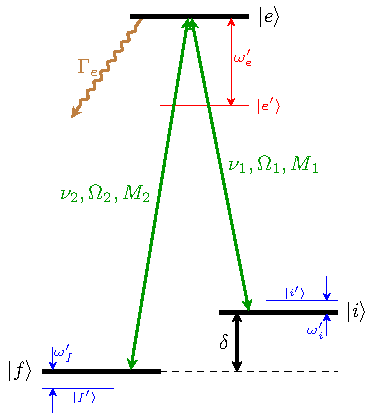
\includegraphics[width=0.6\textwidth]{figures/raman_transfer_generic_stirap_model.pdf}
  \caption[Generic model for a real STIRAP]{
    Generic model for a real STIRAP similar to Fig.~\ref{fig:raman-transfer:generic-raman-model}.
    Differences are that the two beams are now on resonant with $|e\rangle$
    and the $\Omega_1$ and $\Omega_2$ now represent the maximum single photon Rabi frequency
    during the STIRAP pulse for the two beams.
    \label{fig:raman-transfer:generic-stirap-model}}
\end{figure}

\subsection{STIRAP for Ideal Three-Level System}
\label{ch:raman-transfer:stirap:three-level}

During STIRAP, the system approximately remains in a dark state $|D(t)\rangle$
\begin{align*}
  |D(t)\rangle=&c_i(t)|i\rangle+c_f(t)|f\rangle
\end{align*}
Since this state does not couple to the excited state, we have,
\begin{align*}
  0=&\langle e|\mathbf{d}\cdot\mathbf{E}|D(t)\rangle\\
  =&c_i(t)\langle e|\mathbf{d}\cdot\mathbf{E}|i\rangle
     +c_f(t)\langle e|\mathbf{d}\cdot\mathbf{E}|f\rangle\\
  =&c_i(t)\Omega_1(t)+c_f(t)\Omega_2(t)
\end{align*}
or
\begin{align*}
  |D(t)\rangle=&\frac{\Omega_2(t)|i\rangle-\Omega_1(t)|f\rangle}{\sqrt{\Omega_1^2(t)+\Omega_2^2(t)}}
\end{align*}
In order to estimate the scattering rate,
we use the fact that the wavefunction amplitude in the final state $c_f$
is the integral of the excited state amplitude $c_e$ and the down leg Rabi frequency $\Omega_2$,
i.e.,\footnote{This equation and the lower bound on scattering probability applies generically
  to all two photon transfer process including Raman $\pi$ pulse.
  The equation we used in section~\ref{ch:raman-transfer:raman} is a refinement
  on this limit.}
\begin{align*}
  c_f(t)=&\int_0^t \frac{\ui\Omega_2(t)}{2}c_e(t') \ud t'
\end{align*}
For a complete transfer of length $T$, we have $c_f(0)=0$ and $c_f(T)=1$, therefore,
\begin{align*}
  \int_0^T\Omega_2(t)c_e(t)\ud t=&-2\ui
\end{align*}
Since $\Omega_2$ is the upper bound of $\abs{\Omega_2(t)}$ we have,
\begin{align*}
  \abs{\int_0^Tc_e(t)\ud t}\geqslant&\frac{2}{\Omega_2}
\end{align*}
The total scattering probability is,
\begin{align*}
  p_{\mathrm{s}0}=&\int_0^T \Gamma_e|c_e^2(t)| \ud t\\
  \geqslant&\frac{\Gamma_e}{T}\abs{\int_0^T c_e(t) \ud t}^2\\
  \geqslant&\frac{4\Gamma_e}{\Omega_2^2T}
\end{align*}
From similar argument, we also have,
\begin{align*}
  p_{\mathrm{s}0}\geqslant&\frac{4\Gamma_e}{\Omega_1^2T}
\end{align*}
which is the same as the previous result for a three-level STIRAP system
where $\Omega_1=\Omega_2$.
In the generic case, these give us a lower bound on the scattering probability,
\begin{align*}
  \min\paren{p_{\mathrm{s}0}}=&\frac{4\Gamma_e}{\min\paren{\Omega_1^2, \Omega_2^2}T}
\end{align*}
whereas the full scattering is larger than this lower bound by a pulse shape dependent
small constant factor.
It is also easy to verify that this result agrees with the scattering probability for
a optimal three-level Raman $\pi$ with similar single photon Rabi frequency and pulse time.
This confirms that without additional constraint from the real system or the experimental setup,
neither Raman transfer or STIRAP offers a significant advantage over the other.
As we will see in the following sections,
other effects in the system can favor one approach over the other one.

\subsection{Additional Initial and Final States}
\label{ch:raman-transfer:stirap:extra-init-final}

Similar to Raman transition~(section~\ref{ch:raman-transfer:raman:extra-init-final}),
the additional initial and final states causes potential leakage out of the three-level system.
This limits the minimum time of the transfer in a way similar to that of Raman transition.

\subsection{Additional Excited States}
\label{ch:raman-transfer:stirap:extra-ext}

For additional excited states that are farther away than the single photon Rabi frequency
$\Omega_1$ and $\Omega_2$, the contribution to the coherent transfer is minimum.
However, these states can still contribute to scattering during the transfer.

Excited state will only contribute significantly to the scattering if it causes scattering
from the dark state, which happens if $\Omega_1(t)/\Omega_2(t)\neq\Omega'_1(t)/\Omega'_2(t)$,
where $\Omega'_1(t)$ and $\Omega'_2(t)$ are the time dependent single photon Rabi frequencies
coupling $|e'\rangle$ to $|i\rangle$ and $|f\rangle$ respectively.
As discussed in section~\ref{ch:raman-transfer:raman:extra-ext:tight-spacing},
this does not happen for excited state with the same vibrational and electronic states
when the initial and final spin and rotational states are identical.
Similar to $\Omega_1$ and $\Omega_2$, we can also define
$\Omega'_1\equiv\max\paren{\Omega'_1(t)}$ and $\Omega'_2\equiv\max\paren{\Omega'_2(t)}$.
Since $\Omega'_1(t)$($\Omega'_2(t)$) and $\Omega_1(t)$($\Omega_2(t)$)
are generated from the same beam, we have
$\Omega'_1(t)\propto\Omega_1(t)$($\Omega'_2(t)\propto\Omega_2(t)$)
and the condition can also be equivalently expressed as
$\Omega_1/\Omega_2\neq\Omega'_1/\Omega'_2$.

More quantitatively,
the Rabi frequency coupling the dark state $|D(t)\rangle$ to the excited state $|e'\rangle$ is,
\begin{align*}
  \Omega'(t)=&\langle e'|\mathbf{d}\cdot\mathbf{E}|D(t)\rangle\\
  =&\frac{\Omega_2(t)\Omega'_1(t)-\Omega_1(t)\Omega'_2(t)}{\sqrt{\Omega_1^2(t)+\Omega_2^2(t)}}\\
  =&\frac{\Omega_1(t)\Omega_2(t)}{\sqrt{\Omega_1^2(t)+\Omega_2^2(t)}}\paren{\frac{\Omega'_1}{\Omega_1}-\frac{\Omega'_2}{\Omega_2}}
\end{align*}
The addtional scattering caused by this is,
\begin{align*}
  p'_{\mathrm{s}}=&\int_0^T \frac{\Gamma'_e\Omega'^2(t)}{4{\omega'_e}^2} \ud t\\
  =&\frac{\Gamma'_e}{4{\omega'_e}^2}
     \paren{\frac{\Omega'_1}{\Omega_1}-\frac{\Omega'_2}{\Omega_2}}^2
     \int_0^T \frac{\Omega_1^2(t)\Omega_2^2(t)}{\Omega_1^2(t)+\Omega_2^2(t)} \ud t\\
  =&C'\frac{\Gamma'_eT}{4{\omega'_e}^2}
     \paren{\frac{\Omega'_1}{\Omega_1}-\frac{\Omega'_2}{\Omega_2}}^2
     \frac{\Omega_1^2\Omega_2^2}{\Omega_1^2+\Omega_2^2}
\end{align*}
which has the form of an off-resonance scattering probability.
$C'$ is a dimensionless number depending only on the pulse shape defined as
\begin{align*}
  C'\equiv&\frac{\Omega_1^2+\Omega_2^2}{\Omega_1^2\Omega_2^2T}\int_0^T \frac{\Omega_1^2(t)\Omega_2^2(t)\ud t}{\Omega_1^2(t)+\Omega_2^2(t)}
\end{align*}

It is worth noting that although there aren't two different cases similar to
the discussion for Raman transition in section~\ref{ch:raman-transfer:raman:extra-ext}
due to the lack of detuning in STIRAP,
the difference between excited states with different spacings may still play an important role
when comparing Raman transition to STIRAP.
This is discussed breifly at the end of
section~\ref{ch:raman-transfer:stirap:raman-vs-stirap:extra-ext}.

\subsection{Cross Coupling Between Light Addressing Initial and Final States}
\label{ch:raman-transfer:stirap:cross-couple}

As is the case for Raman transition~(section~\ref{ch:raman-transfer:raman:cross-couple}),
the coupling of each beam on the other initial or final state can cause increased scattering.
The total scattering probability caused by the cross coupling is
\footnote{Here we are making the same assumption of identical matrix elements for the two beams
  as the one we made for Raman transition in section~\ref{ch:raman-transfer:raman:cross-couple}.},
\begin{align*}
  p''_{\mathrm{s}}=&\int_0^T \frac{\Gamma_e\Omega_1^2(t)}{4M_1^2}\frac{M_2^2}{\delta^2}\abs{c_f(t)}^2+\frac{\Gamma_e\Omega_2^2(t)}{4M_2^2}\frac{M_1^2}{\delta^2}\abs{c_i(t)}^2 \ud t\\
  =&\frac{\Gamma_e}{4\delta^2}\int_0^T \frac{M_2^2}{M_1^2}\frac{\Omega_1^4(t)}{\Omega_1^2(t)+\Omega_2^2(t)}+\frac{M_1^2}{M_2^2}\frac{\Omega_2^4(t)}{\Omega_1^2(t)+\Omega_2^2(t)} \ud t\\
  =&\frac{\Gamma_eT}{4\delta^2}\paren{C''_1\frac{M_2^2}{M_1^2}\frac{\Omega_1^4}{\Omega_1^2+\Omega_2^2}+C''_2\frac{M_1^2}{M_2^2}\frac{\Omega_2^4}{\Omega_1^2+\Omega_2^2}}
\end{align*}
where $C''_1$ and $C''_2$ are two dimentionless numbers
depending only on the pulse shape defined as,
\begin{align*}
  C''_i\equiv&\frac{\Omega_1^2+\Omega_2^2}{\Omega_i^4T}\int_0^T \frac{\Omega_i^4(t) \ud t}{\Omega_1^2(t)+\Omega_2^2(t)}
\end{align*}

\subsection{Raman Transfer versus STIRAP}
\label{ch:raman-transfer:stirap:raman-vs-stirap}

As one may expect, the scattering probability and the efficiency of a STIRAP transfer
depends on the precise pulse shape used.
While it may be possible to construct a STIRAP pulse shape
with significantly different constant values,
we will focus our discussion on more traditional shapes and assume
$C''_1\approx C''_2\approx C'\approx1$.

We will compare the scattering probability during STIRAP to that of
Raman $\pi$ pulse in two limiting case depending on whether the contribution
from the additional excited or ground state are more significant.

\subsubsection{More Significant Contribution from Additional Excited State}
\label{ch:raman-transfer:stirap:raman-vs-stirap:extra-ext}

This is the case where excited state separation $\omega_e'$ is significantly smaller compared
to the ground state separation $\delta$.
By choosing an optimal pulse time, the minimum scattering probability for the STIRAP is,
\begin{align*}
  p_{\mathrm{s}}^{\mathrm{STIRAP}}\approx&2\sqrt{\frac{4\Gamma_e}{\min\paren{\Omega_1^2, \Omega_2^2}}\frac{\Gamma'_e}{4{\omega'_e}^2}\paren{\frac{\Omega'_1}{\Omega_1}-\frac{\Omega'_2}{\Omega_2}}^2\frac{\Omega_1^2\Omega_2^2}{\Omega_1^2+\Omega_2^2}}\\
  =&\frac{\sqrt{\Gamma_e\Gamma'_e}}{\omega'_e}
     \abs{\frac{\Omega'_1}{\Omega_1}-\frac{\Omega'_2}{\Omega_2}}
     \frac{2\max\paren{\Omega_1, \Omega_2}}{\sqrt{\Omega_1^2+\Omega_2^2}}\\
  \geqslant&\frac{\sqrt{\Gamma_e\Gamma'_e}}{\omega'_e}
             \abs{\frac{\Omega'_1}{\Omega_1}-\frac{\Omega'_2}{\Omega_2}}
\end{align*}
For Raman $\pi$ pulse,
\begin{align*}
  p_{\mathrm{s}}^{\mathrm{Raman}}=&\frac{\pi\Gamma}{2\Omega_{\mathrm{R}}}\\
  =&\frac{\pi}{2}\frac{\Gamma_e\paren{\Omega_1^2+\Omega_2^2}}{4\Delta_{\max}^2}
     \frac{2\Delta_{\max}}{\Omega_1\Omega_2}\\
  =&\frac{\pi\Gamma_e}{4\Delta_{\max}}\frac{\paren{\Omega_1^2+\Omega_2^2}}{\Omega_1\Omega_2}\\
  \geqslant&\frac{\pi\Gamma_e}{2\Delta_{\max}}
\end{align*}
The last inequality for both take the equal sign when $\Omega_1=\Omega_2$.
Comparing the result and note that $\Delta_{\max}$ is a fraction of $\omega_e'$,
we see that the two scales similarly to the excited state spacing.
However, given that in the common cases we have $\Delta_{\max}<\omega_e'$ and
$\abs{\Omega'_1/\Omega_1-\Omega'_2/\Omega_2}<1$ using STIRAP can potentially reduce
the total scattering in this case.

Note that the discussion above implicitly assumes that the relevant $\omega_e'$
is the same for Raman transition and STIRAP.
However, as we saw in section~\ref{ch:raman-transfer:stirap:extra-ext} and
\ref{ch:raman-transfer:raman:extra-ext:tight-spacing},
this may not be the case for hyperfine and rotational structure
in the excited state when the initial and final states have different spin states.
The $\omega_e'$ for STIRAP in this case is the hyperfine or rotational splitting
and may be significantly smaller compared to the $\omega_e'$ for Raman transition,
which is the vibrational state spacing.
As a result, STIRAP may not be as favorable compared to Raman anymore.
The best option in this case would require more in-depth comparison
of the different effects and will not be discussed here in more detail
since it is not relevant in our experiment.

\subsubsection{More Significant Contribution from Additional Ground State}
\label{ch:raman-transfer:stirap:raman-vs-stirap:cross-couple}

With the assumption of $C''_1\approx C''_2\approx1$ the scattering due to
cross coupling for STIRAP is now,
\begin{align*}
  p''_{\mathrm{s}}=&\frac{\Gamma_eT}{4\delta^2}\paren{\frac{M_2^2}{M_1^2}\frac{\Omega_1^4}{\Omega_1^2+\Omega_2^2}+\frac{M_1^2}{M_2^2}\frac{\Omega_2^4}{\Omega_1^2+\Omega_2^2}}\\
  \geqslant&\frac{\Gamma_eT}{2\delta^2}\paren{\Omega_1^2+\Omega_2^2}\frac{M_1^2M_2^2}{\paren{M_1^2+M_2^2}^2}
\end{align*}
and the minimum is taken when $M_2/M_1=\Omega_2/\Omega_1$\footnote{Same as Raman transition.}
The minimum total scattering rate for STIRAP is therefore,
\begin{align*}
  p_{\mathrm{s}}^{\mathrm{STIRAP}}\approx&2\sqrt{\frac{4\Gamma_e}{\min\paren{\Omega_1^2, \Omega_2^2}}\frac{\Gamma_e}{2\delta^2}\paren{\Omega_1^2+\Omega_2^2}\frac{M_1^2M_2^2}{\paren{M_1^2+M_2^2}^2}}\\
  =&2\sqrt{2}\frac{\Gamma_e}{\delta}\frac{M_1M_2}{M_1^2+M_2^2}\frac{\sqrt{\Omega_1^2+\Omega_2^2}}{\min\paren{\Omega_1, \Omega_2}}\\
  =&2\sqrt{2}\frac{\Gamma_e}{\delta}\frac{\max\paren{M_1, M_2}}{\sqrt{M_1^2+M_2^2}}\approx2\sqrt{2}\frac{\Gamma_e}{\delta}
\end{align*}
For Raman transition
\begin{align*}
  p_{\mathrm{s}}^{\mathrm{Raman}}=&\frac{\pi\Gamma}{2\Omega_{\mathrm{R}}}\\
  =&\frac{\pi\Gamma_e}{2\Delta}\frac{M_1^2+M_2^2}{M_1M_2}\\
  \approx&\frac{\pi\Gamma_e}{2\Delta}\frac{\max\paren{M_1,M_2}}{\min\paren{M_1,M_2}}
\end{align*}
we can see that when the single photon Rabi frequency is changed to minimize
cross coupling scattering, the Raman transition can be more strongly affected by
the matrix element imbalance. However, if the Raman transition can use a detuning
\[
  \Delta>\frac{\max\paren{M_1,M_2}}{\min\paren{M_1,M_2}}\delta
\]
then the scattering probability for a Raman transition can be made smaller than that of STIRAP.

\subsubsection{Conclusion}

In our experiment, we have an initial and final state separation of $< 1~\mathrm{GHz}$
and an matrix element ratio of $< 30$.
This means that as long as we can use a single photon detuning of more than
$\approx 30~\mathrm{GHz}$, the total scattering probability for Raman transition
will be smaller than that of STIRAP.
Since this detuning can be achieved easily,
a Raman $\pi$ pulse should be preferred in our experiment.

The comparison so far has been focused on the scattering probability from the Raman or STIRAP
beams. There are also a few other more technical reasons we preferred Raman versus STIRAP
in our experiment.

\begin{enumerate}
\item We use the tweezer beam as the Raman beam for transfer in order to reduce scattering
  from external sources~(section~\ref{ch:raman-spectroscopy:states}).
  Doing this for STIRAP while optimizing the pulse shape for transfer is more challenging.
\item In additional to scattering, the additional excited and ground state
  also causes a power, and therefore time, dependent light shift.
  A STIRAP in the presence of these shifts must vary the frequency of the two beams
  in additional to the power in order to maintain the dark state.
  This is also technically challenging to do.
\end{enumerate}

As a summary, for two photon transfer to a weakly bound molecular state,
it is likely that Raman transition is the preferred technique.
However, for transfering to a deeply bound molecular state,
which is where STIRAP is used in previous experiments,
STIRAP can have an advantage over Raman transition.

\section{States Selection}
\label{ch:raman-transfer:state-selction}

From section~\ref{ch:raman-transfer:raman} we see that the transfer efficiency
is directly related to the excited state linewidth, the maximum usuable detuning
and the matrix elements ratio~($M_1/M_2$).
In this section, we will discuss how these, as well as other technical constraints
affects the choices of states we use for the Raman transfer.

\subsection{Initial Atomic State}
\label{ch:raman-transfer:state-selction:init}

\begin{figure}
  \centering
  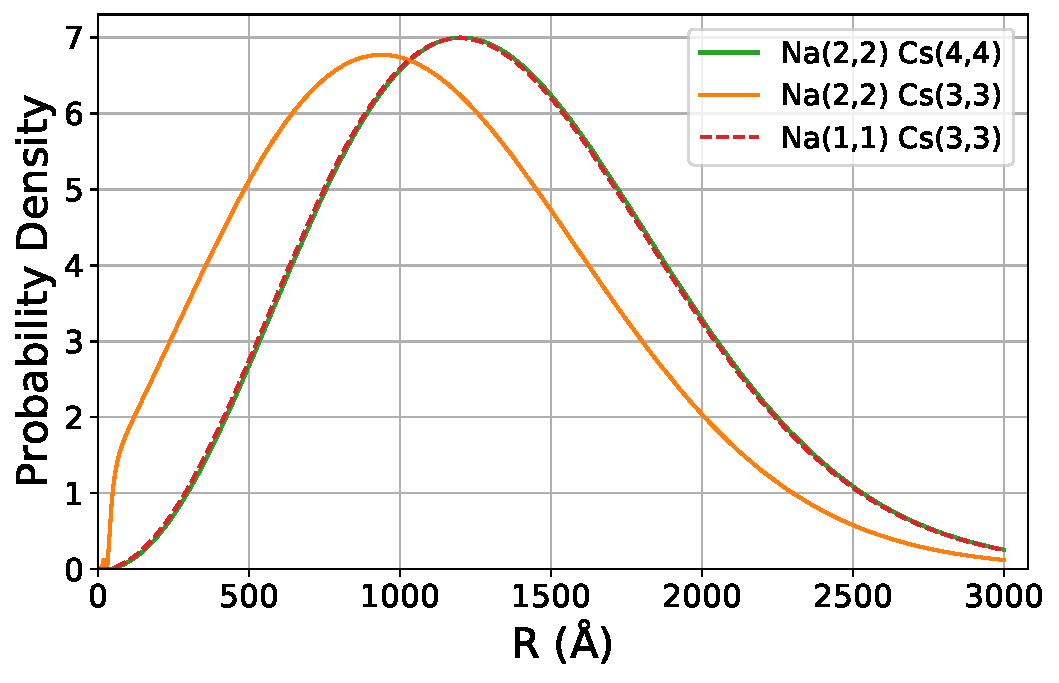
\includegraphics[width=0.625\textwidth]{figures/raman_transfer_atomic_wavefunction.pdf}
  \caption[Enhancement of short range wavefunction]{
    Enhancement of short range wavefunction.
    The large scattering length for the $\mathrm{Na(2,2),Cs(3,3)}$ state
    creates an interaction shift comparable to the axial trapping frequency.
    This causes a significant change in the relative wavefunction especially at short
    intranuclear distance~($R$).
    Compared to other spin states with weaker interaction,
    the wavefunction at short distance~($R<100~\text{\AA}$) is significantly enhanced.
    \label{fig:raman-transfer:atomic-wavefunction}}
\end{figure}

The choice of initial state can affect the transfer efficiency
by changing the matrix element $M_1$ and therefore the matrix elements ratio.
Since for most choices of the atomic and molecular states we have $M_1<M_2$,
we would like to choose an atomic initial state with the largest $M_1$ possible.
Unlike the selection of final state~(section~\ref{ch:raman-transfer:state-selction:final})
maximizing $M_1$ can improve the matrix element ratio as well as
shortening the transfer time to decrease sensitivity to technical noise at the same time.

As discussed in section~\ref{ch:pa:linewidth},
$M_1$ is only sensitive to the wavefunction at a short inter-atomic distance
that is comparable to the size of the molecule.
Therefore, states with a large wavefunction value at short inter-atomic distance
should generally have a larger $M_1$.
In additional to the confinement potential and the motional state of the atoms,
this is also affected by the interaction between the atoms.
A stronge interaction, either attractive or repulse,
can significantly change the relative motional wavefunction of the atoms.
This effect can be seen in Fig.~\ref{fig:raman-transfer:atomic-wavefunction}
and is especially significant for the $|\mathrm{Na(2,2),Cs(3,3)}\rangle$ state
when the interaction energy scale is comparable to that of the motional energy
as seen in section~\ref{ch:interaction-shift:spectroscopy:results}.

\subsection{Excited State}
\label{ch:raman-transfer:state-selction:ext}

\begin{figure}
  \centering
  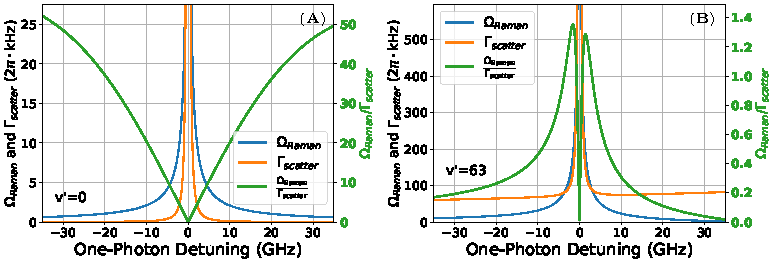
\includegraphics[width=\textwidth]{figures/raman_transfer_v0_vs_v63.pdf}
  \caption[Comparison between using a weakly bound and a deeply bound excited state
  as intermediate state for the Raman transition]{
    Comparison between using a weakly bound and a deeply bound excited state
    as intermediate state for the Raman transition.
    The (A) deeply bound excited state~($v'=0$) has a smaller
    Raman Rabi frequency`($\Omega_{\mathrm{R}}$) compared to the
    (B) weakly bound excited state~($v'=63$) at a given detuning.
    However, the lower scattering rate~($\Gamma_{\mathrm{s}}$) allows a much larger
    $\Delta_{\max}$,
    which results in a larger Raman Rabi frequency to scattering rate ratio.
    \label{fig:raman-transfer:v0-vs-v63}}
\end{figure}

Based on theory calculation, most of the molecular excited states have a linewidth $\Gamma_e'$
very similar to that of the Cesium D lines between $2\pi\times5~\mathrm{MHz}$ to
$2\pi\times10~\mathrm{MHz}$ due to optical decay process.
States above the Cesium $\mathrm{6^2P_{1/2}}$ state,
however, could non-radiatively decay to the Cs $\mathrm{6^2P_{1/2}}$
and Na $\mathrm{3^2S_{1/2}}$ states
via pre-dissociation which significantly increases the linewidth and should be avoided.

The other factor that affects excited state selection is the maximum detuning $\Delta_{\max}$.
Due to larger FCF with the ground atomic and weakly bound molecular state,
previous attempt at Raman spectroscopy typically use an excited state
closed to the dissociative threshold as
the intermediate state~\cite{wynar_molecules_2000,rom_state_2004}.
However, the smaller inter-state spacing and the smaller detuning from
the atomic excited state means that these state have a relatively small $\Delta_{\max}$
and therefore a lower coherent transfer efficiency.
On the other hand, a deeply bound excited state has a significantly higher $\Delta_{\max}$
and is the preferred choice for coherent Raman transfer.

In the experiment, we use numerical simulation to calculate the Raman transfer efficiency
for any given Raman beam wavelength taking into account of all states of
the $\mathrm{c^3\Sigma^+}(\Omega = 1)$
excited molecular state potential~\cite{grochola_spin-forbidden_2011}
and the continuum~\cite{liu_ultracold_2017}.
Fig.~\ref{fig:raman-transfer:v0-vs-v63} shows the result near a deeply bound
and weakly bound excited state.
Despite having a lower Raman Rabi frequency,
the deeply bound state has significantly higher transfer efficiency
and is used as the intermediate state for coherent Raman transfer in our experiment.

\subsection{Final Molecular State}
\label{ch:raman-transfer:state-selction:final}

In additional to the scattering and light shift considertions discussed above,
the transition can also be affected by external magnetic field.
We minimize the effect of magnetic field noise on the transition by using molcular
and atomic states that are in the same molecular potential,
i.e. molecular bound state in the potential that asymptote to
the atomic state. For weakly bound molecular state,
i.e. binding energy smaller than or comparable to the hyperfine energy scale,
this ensures that the atomic and molecular states has maximally overlapping spin state
and therefore a small differential Zeeman shift that can affect the Raman resonance frequency.
The similarity in the spin state between the initial and final states
also minimizes the effect of hyperfine and rotational states near the excited states
as we have seen in section~\ref{ch:raman-transfer:raman:extra-ext:tight-spacing}.

Because of the weak coupling between the atomic and molecular states,
the Raman transition has a relatively low Rabi frequency.
This also means a longer transfer time over which the Raman lasers must remain coherent.
In order to lower the requirement on our Raman and tweezer laser,
we select the first bound state, i.e. smallest binding energy, as the final molecular state.
This ensures the maximum Raman Rabi frequency.
Additionally, the typical binding energy for these states are $<1~\mathrm{GHz}$
which is a frequency difference that can be generated using AOM's
so that the coherence between the two beams is greatly improved.

\section{Raman Transfer Results}
\label{ch:raman-transfer:results}

The setup and sequence for forming the molecule is very similar to that of the Raman spectsocopy
previously mentioned in section~\ref{ch:raman-spectroscopy:states:raman-tweezer}
that drives the two-photon transition by adding a second frequency to the tweezer light.
Nevertheless, a few changes were made to the sequence in order to improve
the transfer efficiency and the signal to noise.
\begin{enumerate}
\item The initial $|\mathrm{Na(2,2),Cs(3,3)}\rangle$ state is prepared by driving the
  interaction shift resonance from $|\mathrm{Na(2,2),Cs(4,4)}\rangle$
  after the two atoms are merged into the same tweezer.
  As discussed in section~\ref{ch:interaction-shift:summary},
  the strong interaction between the atoms allows preparation of
  relative motional ground state with low background.
\item Instead of using smaller detuning and longer time to maximize the signal of the resonance,
  we increased the single photon detuning to $145~\mathrm{GHz}$
  and use short pulse times~($<1~\mathrm{ms}$)
  to reduce the scattering and the linewidth of the resonance.
\item We added an narrow bandpass filter to reduce the spectral noise from the laser.
  This will be discussed in more detail below.\todo{ref}
\end{enumerate}

With these changes, the narrowest linewidth we were able to observe using $15~\mathrm{mW}$
of total power in the tweezer is shown in Fig.~\todo{ref, data using one ASE filter}.
The full width half maximum~(FWHM) of $\todo{number}~\mathrm{kHz}$ is consistent
with the Fourier limited linewidth of $\todo{number}~\mathrm{kHz}$
for a $\pi$-pulse of $\todo{number}~\mathrm{ms}$ used in the experiment.
This is evidence that the linewidth is mainly determined by the Raman Rabi frequency
rather than the lifetime of the molecule, suggesting that we are in the coherent regime.
We can confirm this by varying the pulse time on the Raman resonance
and the resulting decaying Rabi flopping can be seen in Fig.~\todo{ref}.

\todo{
  Lower than expected efficiency
  Scan dependency of parameters to determine the cause
}

\subsection{Effect of laser spectral noise}
\label{ch:raman-transfer:results:ase}

\subsection{Scaling of Raman Transition Parameters}
\label{ch:raman-transfer:results:scaling}

\todo{
  Types of sources: one/two photon
  Background/v=0 contribution
}

\section{Summary and Outlook}
\label{ch:raman-transfer:summary}

\todo{
  Reference loss due to coupling to atomic motional continuum
}


(outlook:)

Since the final state is mainly selected based on technical considerations,
there are other choices that can potentially improve the transfer efficiency.
As an exmple, states with larger binding energies can have weaker coupling
to the excited state therefore reducing the matrix elements ratio.
Doing so would likely require locking two lasers with a coherence time
longer than a few milliseconds.
